\let\negmedspace\undefined
\let\negthickspace\undefined
\documentclass[journal]{IEEEtran}
\usepackage[a5paper, margin=10mm, onecolumn]{geometry}
\usepackage{lmodern} % Ensure lmodern is loaded for pdflatex
\usepackage{tfrupee} % Include tfrupee package

\setlength{\headheight}{1cm} % Set the height of the header box
\setlength{\headsep}{0mm}     % Set the distance between the header box and the top of the text

\usepackage{gvv-book}
\usepackage{gvv}
\usepackage{cite}
\usepackage{amsmath,amssymb,amsfonts,amsthm}
\usepackage{algorithmic}
\usepackage{graphicx}
\usepackage{textcomp}
\usepackage{xcolor}
\usepackage{txfonts}
\usepackage{listings}
\usepackage{enumitem}
\usepackage{mathtools}
\usepackage{gensymb}
\usepackage{comment}
\usepackage[breaklinks=true]{hyperref}
\usepackage{tkz-euclide} 
\usepackage{listings}
% \usepackage{gvv}                                        
\def\inputGnumericTable{}                                 
\usepackage[latin1]{inputenc}                                
\usepackage{color}                                            
\usepackage{array}                                            
\usepackage{longtable}                                       
\usepackage{calc}                                             
\usepackage{multirow}                                         
\usepackage{hhline}                                           
\usepackage{ifthen}                                           
\usepackage{lscape}
\begin{document}

\bibliographystyle{IEEEtran}
\vspace{3cm}

\title{1.15.29}
\author{EE24BTECH11005 - Arjun Pavanje
}
% \maketitle
% \newpage
% \bigskip
{\let\newpage\relax\maketitle}

\textbf{Question}:\\
The coordinates of the point \textbf{P} dividing the line segment joining the points \textbf{A}(1,3) and \textbf{B}(4,6) in the ratio 2:1 are
\hfill (10, 2012)
\\
\textbf{Solution: }
\begin{table}[h!]    
  \centering
  \begin{tabular}[12pt]{ |c| c|}
    \hline
    \textbf{Variable} & \textbf{Description}\\ 
    \hline
	$\vec{a}$ & $BC$ line\\
   \hline
	$\vec{b}$ & $AC$ line\\
   \hline
	$\vec{c}$ & $AB$ line, $5cm$ length\\
   \hline
	$\vec{K}$ & $a+b=5cm$\\
	\hline
	$\vec{\angle{A}}$ & $\angle{BAC}=45{\degree}$\\
	\hline

    \end{tabular}

  \caption{Variables Used}
  \label{tab1.15.29}
\end{table}
If $P$ divides $AB$ in the ratio $k:1$,


\begin{align} 
\textbf{P}=\frac{k\textbf{C}+\textbf{B}}{k+1} \label{eq1.15.29.1}\\
\end{align}
From equation \ref{eq1.15.29.1} we have
\begin{align}
P &= \frac{k
\myvec{
1\\
3} +
\myvec{
4\\
6}}{k+1} \label{eq1.15.29.2}\\
&= \frac{
\myvec{
k+4 \\
3k+6
}}{k+1} \label{eq1.15.29.3}
\end{align}
here, $k = 2$, so putting the $k$ value into \ref{eq1.15.29.3} we get
\begin{align}
P &= \frac{
\myvec{
6\\
12
}}{3} \label{eq1.15.29.4}\\
&=
\myvec{
2\\
4
	} \label{eq1.15.29.5}
\end{align}
The coordinates of the required point $P$ are
\myvec{
2\\
4
}
\begin{figure}[h!]
   \centering
   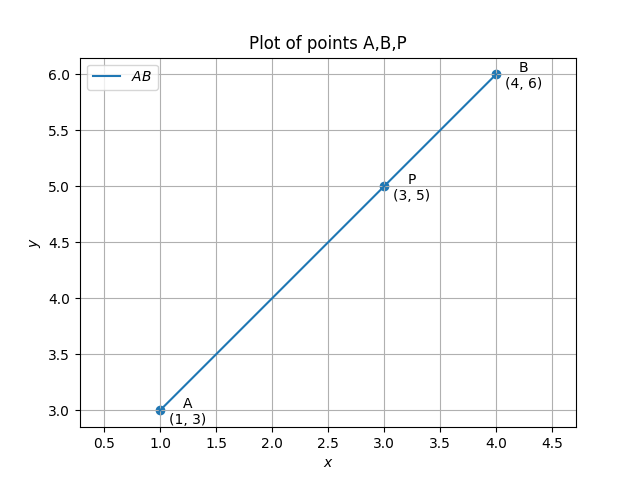
\includegraphics[width=0.7\linewidth]{figs/Figure_1.png}
   \caption{Plot of the points A,B,P}
   \label{stemplot}
\end{figure}
\end{document}
